% !TeX program = xelatex
\documentclass[a4paper,10pt]{article}

% ============================================================================
% កញ្ចប់បណ្ណាល័យ (Packages) – តាមលំនាំស្តង់ដារអនុវិទ្យាល័យព្រះក្រសាំង (ls_plan.tex)
% ============================================================================
\usepackage[a4paper, left=0.95cm, right=0.95cm, top=0.85cm, bottom=0.92cm, footskip=0.52cm]{geometry}
\usepackage{amsmath}
\usepackage{unicode-math}
\usepackage{fontspec}
\usepackage{array, longtable, multirow, colortbl}
\usepackage[table]{xcolor}
\usepackage{enumitem}
\usepackage{pifont}
\usepackage{fancyhdr}
\usepackage{tikz}
\usetikzlibrary{calc, arrows.meta, angles, quotes, decorations.markings, babel}

% LaTeX 2025 + longtable compatibility guard
\makeatletter
\let\@expl@@@mark@update@singlecol@structures@@\relax
\makeatother

% ============================================================================
% ការកំណត់ពុម្ពអក្សរ (Cross-Platform Windows + Linux Cloud fonts/)
% ============================================================================
\providecommand{\NGSFindFonts}{%
  \IfFileExists{C:/Windows/Fonts/cambria.ttc}{%
    \def\NGSSysPath{C:/Windows/Fonts/}%
    \def\NGSUserPath{C:/Users/KIT/AppData/Local/Microsoft/Windows/Fonts/}%
  }{%
    \IfFileExists{./fonts/KhmerOSsiemreap.ttf}{\def\NGSSysPath{./fonts/}\def\NGSUserPath{./fonts/}}{%
    \IfFileExists{../fonts/KhmerOSsiemreap.ttf}{\def\NGSSysPath{../fonts/}\def\NGSUserPath{../fonts/}}{%
    \IfFileExists{../../fonts/KhmerOSsiemreap.ttf}{\def\NGSSysPath{../../fonts/}\def\NGSUserPath{../../fonts/}}{%
    \IfFileExists{../../../fonts/KhmerOSsiemreap.ttf}{\def\NGSSysPath{../../../fonts/}\def\NGSUserPath{../../../fonts/}}{%
    \IfFileExists{../../../../fonts/KhmerOSsiemreap.ttf}{\def\NGSSysPath{../../../../fonts/}\def\NGSUserPath{../../../../fonts/}}{%
    \IfFileExists{../../../../../fonts/KhmerOSsiemreap.ttf}{\def\NGSSysPath{../../../../../fonts/}\def\NGSUserPath{../../../../../fonts/}}{%
    \IfFileExists{../../../../../../fonts/KhmerOSsiemreap.ttf}{\def\NGSSysPath{../../../../../../fonts/}\def\NGSUserPath{../../../../../../fonts/}}{%
      \def\NGSSysPath{../../../../../../../fonts/}\def\NGSUserPath{../../../../../../../fonts/}%
    }}}}}}}%
  }%
}
\NGSFindFonts

\setmathfont[
  Path={\NGSSysPath},
  FontIndex=1,
  Scale=1.02
]{cambria.ttc}

\defaultfontfeatures{Ligatures=TeX}

\setmainfont[
  Path={\NGSUserPath},
  Extension=.ttf,
  Script=Khmer,
  BoldFont={KhmerOSsiemreap},
  BoldFeatures={FakeBold=1.8},
  ItalicFont={KhmerOSsiemreap},
  ItalicFeatures={FakeSlant=0.25},
  BoldItalicFont={KhmerOSsiemreap},
  BoldItalicFeatures={FakeBold=1.8, FakeSlant=0.25}
]{KhmerOSsiemreap}

\newfontfamily\muol[
  Path={\NGSUserPath},
  Extension=.ttf,
  Script=Khmer
]{KhmerOSmuollight}

\newfontfamily\TimesEn[
  Path={\NGSSysPath},
  Extension=.ttf,
  Scale=1.00,
  BoldFont={timesbd},
  ItalicFont={timesi},
  BoldItalicFont={timesbi}
]{times}

\newfontfamily\NagaBold[
  Path={\NGSUserPath},
  Extension=.ttf
]{AKbalthom Naga Bold}

\newfontfamily\CalibriFont[
  Path={\NGSSysPath},
  Extension=.ttf
]{calibri}

\newfontfamily\Tacteing[
  Path={\NGSUserPath}
]{TACTENG.TTF}

\newfontfamily\CourierBullet[
  Path={\NGSSysPath},
  Extension=.ttf
]{cour}
\newcommand{\wcirc}{{\CourierBullet\fontsize{9.5pt}{11pt}\selectfont o}}

\XeTeXlinebreaklocale "km"
\XeTeXlinebreakskip = 0pt plus 1pt minus 0.1pt

% ============================================================================
% ពណ៌ និងទម្រង់ទំព័រ
% ============================================================================
\definecolor{stepgray}{HTML}{D9D9D9}
\definecolor{headgray}{HTML}{F2F2F2}
\definecolor{boxgray}{HTML}{E6E6E6}
\definecolor{darkred}{HTML}{C00000}
\definecolor{red5e}{HTML}{FF0000}

\pagestyle{fancy}
\fancyhf{}
\renewcommand{\headrulewidth}{0pt}
\fancyfoot[R]{\CalibriFont\fontsize{11pt}{13pt}\selectfont\thepage}

\setlength{\parindent}{0pt}
\setlength{\parskip}{0pt}
\setlength{\tabcolsep}{3.8pt}

\newcolumntype{L}[1]{>{\raggedright\arraybackslash}p{#1}}

% ============================================================================
% ម៉ាក្រូជំនួយ (Helper Macros)
% ============================================================================
\newcommand{\en}[1]{{\TimesEn #1}}
\newcommand{\enbf}[1]{{\TimesEn\textbf{#1}}}
\newcommand{\unit}[1]{\,\text{\en{#1}}}
\newcommand{\fiveE}[1]{{\NagaBold\fontsize{9.5pt}{13pt}\selectfont\textcolor{red5e}{#1}}}
\newcommand{\timenote}[1]{\textcolor{darkred}{\textit{#1}}}
\newcommand{\graybox}[1]{\colorbox{boxgray}{\strut\hspace{2pt}#1\hspace{2pt}}}
\newcommand{\ditem}{\tikz[baseline=-0.5ex]\fill (0,0.42ex) -- (0.42ex,0) -- (0,-0.42ex) -- (-0.42ex,0) -- cycle;\hspace{0.3em}}
\newcommand{\cnum}[1]{{\fontsize{10.5pt}{12pt}\selectfont\ding{\numexpr181+#1\relax}}\hspace{0.2em}}
\newcommand{\cfig}[1]{\par\vspace{4pt}{\centering #1\par}\vspace{4pt}}
\newcommand{\stepheader}[1]{\multicolumn{3}{|c|}{\cellcolor{stepgray}\muol #1} \\* \noalign{\hrule height 0.4pt}}
\newcommand{\tri}[1]{\ensuremath{\triangle #1}}
\newcommand{\ang}[1]{\ensuremath{\angle #1}}
\newcommand{\cg}{\ensuremath{\cong}}
\newcommand{\chkbox}{\tikz[baseline=-0.15ex]\draw[black, line width=0.8pt] (0,0) rectangle (0.23cm,0.23cm);}

\tikzset{
  tk1/.style={postaction={decorate},decoration={markings,mark=at position 0.50 with {\draw[black, line width=0.85pt](0,-0.095)--(0,0.095);}}},
  tk2/.style={postaction={decorate},decoration={markings,
    mark=at position 0.45 with {\draw[black, line width=0.85pt](0,-0.095)--(0,0.095);},
    mark=at position 0.55 with {\draw[black, line width=0.85pt](0,-0.095)--(0,0.095);}}},
  tk3/.style={postaction={decorate},decoration={markings,
    mark=at position 0.42 with {\draw[black, line width=0.85pt](0,-0.095)--(0,0.095);},
    mark=at position 0.50 with {\draw[black, line width=0.85pt](0,-0.095)--(0,0.095);},
    mark=at position 0.58 with {\draw[black, line width=0.85pt](0,-0.095)--(0,0.095);}}}
}

\newcommand{\rightbox}[4][0.19]{%
  \draw[black, line width=0.8pt]
    ($(#3)!#1!(#2)$) -- ($($(#3)!#1!(#2)$)+($(#3)!#1!(#4)$)-(#3)$) -- ($(#3)!#1!(#4)$);
}

\newcommand{\khmflourish}{{\Tacteing\fontsize{36pt}{14pt}\selectfont\raisebox{-5pt}{3}}}

% ============================================================================
% ម៉ាក្រូគូសរូបធរណីមាត្រ B&W ច្បាស់សមាមាត្រ (3.8–6.8 cm, អក្សរខ្មៅ 100%)
% ============================================================================

% ១. រំលឹកមេរៀនចាស់៖ លក្ខណៈមេដ្យាទ័រនៃអង្កត់ និង មេដ្យានត្រីកោណកែងទៅអ៊ីប៉ូតេនុស
\newcommand{\figPrereqPBIS}{%
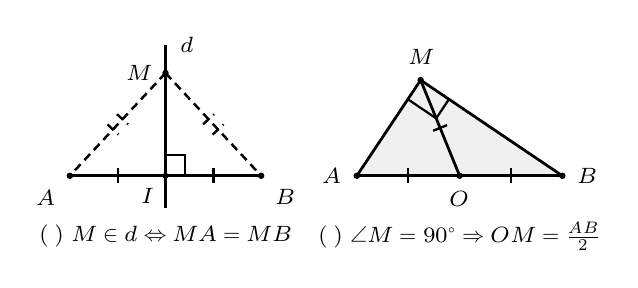
\begin{tikzpicture}[scale=0.90, every node/.style={font=\footnotesize, text=black}]
  % (១) មេដ្យាទ័រ d នៃអង្កត់ AB
  \begin{scope}[shift={(0,0)}]
    \coordinate (A) at (-1.35,0);
    \coordinate (B) at (1.35,0);
    \coordinate (I) at (0,0);
    \coordinate (M) at (0,1.45);
    \draw[black, line width=1.0pt, tk1] (A) -- (I);
    \draw[black, line width=1.0pt, tk1] (I) -- (B);
    \draw[black, line width=1.0pt] (0,-0.45) -- (0,1.85) node[right=1.5pt] {$d$};
    \draw[black, line width=0.9pt, densely dashed, tk2] (M) -- (A);
    \draw[black, line width=0.9pt, densely dashed, tk2] (M) -- (B);
    \rightbox[0.20]{M}{I}{B}
    \fill[black] (A) circle (1.3pt) node[below left=1.5pt] {$A$};
    \fill[black] (B) circle (1.3pt) node[below right=1.5pt] {$B$};
    \fill[black] (I) circle (1.2pt) node[below left=1pt] {$I$};
    \fill[black] (M) circle (1.3pt) node[left=2pt] {$M$};
    \node at (0,-0.85) {(១) $M\in d \Leftrightarrow MA=MB$};
  \end{scope}
  % (២) ត្រីកោណកែង មេដ្យានទៅអ៊ីប៉ូតេនុស
  \begin{scope}[shift={(4.15,0)}]
    \coordinate (A) at (-1.45,0);
    \coordinate (B) at (1.45,0);
    \coordinate (O) at (0,0);
    \coordinate (M) at (-0.55,1.35);
    \fill[gray!12] (A) -- (M) -- (B) -- cycle;
    \draw[black, line width=1.0pt] (A) -- (M) -- (B);
    \draw[black, line width=1.0pt, tk1] (A) -- (O);
    \draw[black, line width=1.0pt, tk1] (O) -- (B);
    \draw[black, line width=1.0pt, tk1] (M) -- (O);
    \rightbox[0.20]{A}{M}{B}
    \fill[black] (A) circle (1.3pt) node[left=2pt] {$A$};
    \fill[black] (B) circle (1.3pt) node[right=2pt] {$B$};
    \fill[black] (M) circle (1.3pt) node[above=2pt] {$M$};
    \fill[black] (O) circle (1.3pt) node[below=2pt] {$O$};
    \node at (0,-0.85) {(២) $\ang{M}=90^\circ \Rightarrow OM=\frac{AB}{2}$};
  \end{scope}
\end{tikzpicture}}

% ២. E1 Engage: អណ្ដូងទឹករួមស្មើចម្ងាយពីសាលារៀនភូមិទាំង ៣ (A, B, C)
\newcommand{\figEngagePBIS}{%
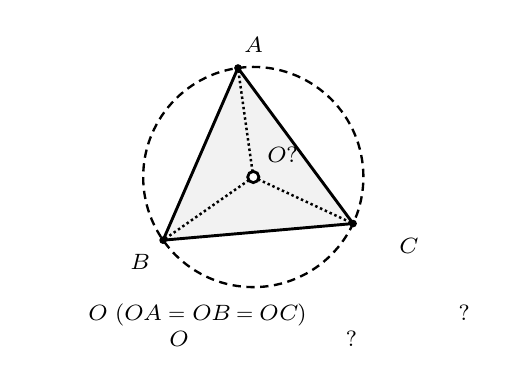
\begin{tikzpicture}[scale=0.92, every node/.style={font=\footnotesize, text=black}]
  \coordinate (O) at (0,0);
  \def\R{1.52}
  \coordinate (A) at (98:\R);
  \coordinate (B) at (215:\R);
  \coordinate (C) at (-25:\R);
  \draw[black, line width=0.85pt, densely dashed] (O) circle (\R);
  \fill[gray!10] (A) -- (B) -- (C) -- cycle;
  \draw[black, line width=1.05pt] (A) -- (B) -- (C) -- cycle;
  \draw[black, line width=0.9pt, densely dotted] (O) -- (A) (O) -- (B) (O) -- (C);
  \fill[black] (A) circle (1.5pt) node[above=2pt] {ភូមិ $A$};
  \fill[black] (B) circle (1.5pt) node[below left=1.5pt] {ភូមិ $B$};
  \fill[black] (C) circle (1.5pt) node[below right=1.5pt] {ភូមិ $C$};
  \fill[white] (O) circle (2.2pt);
  \draw[black, line width=1.0pt] (O) circle (2.2pt);
  \node[above right=1.5pt] at (O) {$O?$};
  \node[align=center] at (0,-2.05) {តើចំណុច $O$ ($OA=OB=OC$) រកតាមមេដ្យាទ័រ ឬមេដ្យាន?\\តើ $O$ នៅក្នុងត្រីកោណជានិច្ចឬទេ?};
\end{tikzpicture}}

% ២ខ. E2 សកម្មភាពទី១៖ ករណីប្រៀបធៀបទាំង ៣ (មុំស្រួច, កែង, មុំទាល)
\newcommand{\figCasesPBIS}{%
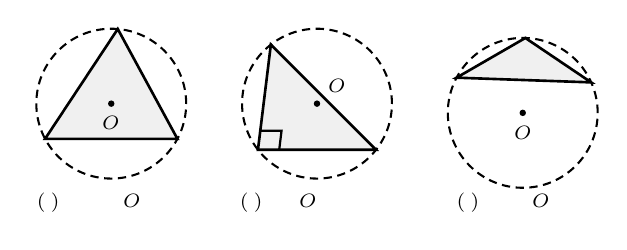
\begin{tikzpicture}[scale=0.78, every node/.style={font=\scriptsize, text=black}]
  % (១) មុំស្រួច៖ O នៅក្នុង
  \begin{scope}[shift={(0,0)}]
    \coordinate (O) at (0,0);
    \def\R{1.22}
    \coordinate (A) at (85:\R);
    \coordinate (B) at (208:\R);
    \coordinate (C) at (-28:\R);
    \draw[black, line width=0.75pt, densely dashed] (O) circle (\R);
    \fill[gray!12] (A) -- (B) -- (C) -- cycle;
    \draw[black, line width=0.95pt] (A) -- (B) -- (C) -- cycle;
    \fill[black] (O) circle (1.5pt) node[below=1pt] {$O$};
    \node at (0,-1.62) {(១) មុំស្រួច៖ $O$ នៅក្នុង};
  \end{scope}
  % (២) កែង៖ O ចំកណ្ដាលអ៊ីប៉ូតេនុស
  \begin{scope}[shift={(3.35,0)}]
    \coordinate (O) at (0,0);
    \def\R{1.22}
    \coordinate (E) at (128:\R);
    \coordinate (D) at (-142:\R);
    \coordinate (F) at (-38:\R);
    \draw[black, line width=0.75pt, densely dashed] (O) circle (\R);
    \fill[gray!12] (D) -- (E) -- (F) -- cycle;
    \draw[black, line width=0.95pt] (D) -- (E) -- (F) -- cycle;
    \rightbox[0.18]{E}{D}{F}
    \fill[black] (O) circle (1.5pt) node[above right=0.5pt] {$O$};
    \node at (0,-1.62) {(២) កែង៖ $O$ លើអ៊ីប៉ូតេនុស};
  \end{scope}
  % (៣) មុំទាល៖ O នៅក្រៅ
  \begin{scope}[shift={(6.70,0)}]
    \coordinate (O) at (0,-0.15);
    \def\R{1.22}
    \coordinate (M) at ($(O)+(88:\R)$);
    \coordinate (N) at ($(O)+(152:\R)$);
    \coordinate (P) at ($(O)+(24:\R)$);
    \draw[black, line width=0.75pt, densely dashed] (O) circle (\R);
    \fill[gray!12] (M) -- (N) -- (P) -- cycle;
    \draw[black, line width=0.95pt] (M) -- (N) -- (P) -- cycle;
    \fill[black] (O) circle (1.5pt) node[below=1pt] {$O$};
    \node at (0,-1.62) {(៣) មុំទាល៖ $O$ នៅក្រៅ};
  \end{scope}
\end{tikzpicture}}

% ៣. E2/E3 ឧទាហរណ៍ និងទ្រឹស្ដីបទ រង្វង់ចារឹកក្រៅត្រីកោណ (ទំ.២០៧)
\newcommand{\figCircumPBIS}{%
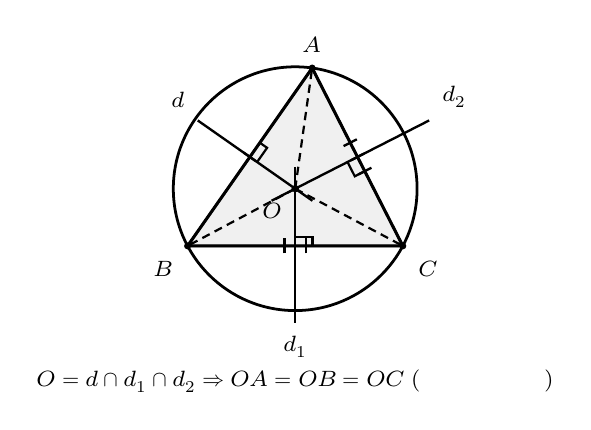
\begin{tikzpicture}[scale=0.90, every node/.style={font=\footnotesize, text=black}]
  \coordinate (O) at (0,0);
  \def\R{1.72}
  \coordinate (A) at (82:\R);
  \coordinate (B) at (208:\R);
  \coordinate (C) at (-28:\R);
  \coordinate (K) at ($(A)!0.5!(B)$);
  \coordinate (M) at ($(B)!0.5!(C)$);
  \coordinate (N) at ($(A)!0.5!(C)$);

  \draw[black, line width=1.0pt] (O) circle (\R);
  \fill[gray!12] (A) -- (B) -- (C) -- cycle;
  \draw[black, line width=1.1pt] (A) -- (B) -- (C) -- cycle;

  % មេដ្យាទ័រ d, d1, d2 លាតចេញក្រៅរង្វង់ឱ្យច្បាស់
  \draw[black, line width=0.85pt] ($(O)!-0.38!(K)$) -- ($(O)!2.15!(K)$) node[above left=1pt] {$d$};
  \draw[black, line width=0.85pt] ($(O)!-0.38!(M)$) -- ($(O)!2.35!(M)$) node[below=1pt] {$d_1$};
  \draw[black, line width=0.85pt] ($(O)!-0.38!(N)$) -- ($(O)!2.15!(N)$) node[above right=1pt] {$d_2$};

  \rightbox[0.16]{O}{K}{A}
  \rightbox[0.16]{O}{M}{C}
  \rightbox[0.16]{O}{N}{C}

  \draw[black, line width=0.8pt, tk1] (A) -- (K) (K) -- (B);
  \draw[black, line width=0.8pt, tk2] (B) -- (M) (M) -- (C);
  \draw[black, line width=0.8pt, tk3] (A) -- (N) (N) -- (C);
  \draw[black, line width=0.8pt, densely dashed] (O) -- (A) (O) -- (B) (O) -- (C);

  \fill[black] (A) circle (1.4pt) node[above=2pt] {$A$};
  \fill[black] (B) circle (1.4pt) node[below left=2pt] {$B$};
  \fill[black] (C) circle (1.4pt) node[below right=2pt] {$C$};
  \fill[black] (O) circle (1.5pt) node[below left=1.5pt] {$O$};
  \node at (0,-2.72) {$O = d \cap d_1 \cap d_2 \Rightarrow OA=OB=OC$ (ផ្ចិតរង្វង់ចារឹកក្រៅ)};
\end{tikzpicture}}

% ៤. E4 លំហាត់គំរូ (ទំ.២០៧) និង ប្រតិបត្តិ (ទំ.២០៨)
\newcommand{\figElaboratePBIS}{%
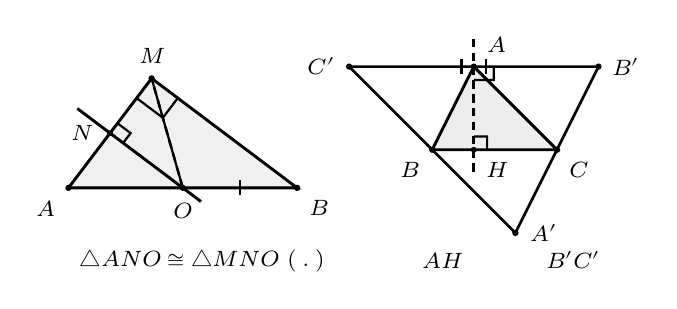
\begin{tikzpicture}[scale=0.88, every node/.style={font=\footnotesize, text=black}]
  % (ក) លំហាត់គំរូ ON មេដ្យាទ័រនៃ AM
  \begin{scope}[shift={(0,0)}]
    \coordinate (A) at (-1.65,0);
    \coordinate (B) at (1.65,0);
    \coordinate (O) at (0,0);
    \coordinate (M) at (-0.45,1.58);
    \coordinate (N) at ($(A)!0.5!(M)$);
    \fill[gray!12] (A) -- (M) -- (B) -- cycle;
    \draw[black, line width=1.05pt] (A) -- (M) -- (B) -- cycle;
    \draw[black, line width=0.9pt, densely dashed] (O) -- (M);
    \draw[black, line width=1.05pt] ($(O)!-0.25!(N)$) -- ($(O)!1.45!(N)$);
    \rightbox[0.18]{A}{M}{B}
    \rightbox[0.18]{O}{N}{M}
    \draw[black, line width=0.8pt, tk1] (A) -- (O) (O) -- (B) (O) -- (M);
    \fill[black] (A) circle (1.3pt) node[below left=1pt] {$A$};
    \fill[black] (B) circle (1.3pt) node[below right=1pt] {$B$};
    \fill[black] (O) circle (1.3pt) node[below=2pt] {$O$};
    \fill[black] (M) circle (1.3pt) node[above=2pt] {$M$};
    \fill[black] (N) circle (1.2pt) node[left=3pt] {$N$};
    \node at (0,-1.05) {គំរូ៖ $\tri{ANO}\cg\tri{MNO}$ (អ.ជ)};
  \end{scope}
  % (ខ) ប្រតិបត្តិ បន្ទាត់ AH ជាមេដ្យាទ័រនៃ B'C'
  \begin{scope}[shift={(4.45,0)}]
    \coordinate (B) at (-0.85,0.55);
    \coordinate (C) at (0.95,0.55);
    \coordinate (A) at (-0.25,1.75);
    \coordinate (Bp) at (1.55,1.75);
    \coordinate (Cp) at (-2.05,1.75);
    \coordinate (Ap) at (0.35,-0.65);
    \coordinate (H) at (-0.25,0.55);
    \fill[gray!14] (A) -- (B) -- (C) -- cycle;
    \draw[black, line width=0.95pt] (Cp) -- (Bp) -- (Ap) -- cycle;
    \draw[black, line width=1.05pt] (A) -- (B) -- (C) -- cycle;
    \draw[black, line width=1.0pt, densely dashed] (-0.25,2.15) -- (-0.25,0.20);
    \rightbox[0.16]{A}{H}{C}
    \rightbox[0.16]{H}{A}{Bp}
    \draw[black, line width=0.8pt, tk2] (Cp) -- (A) (A) -- (Bp);
    \fill[black] (A) circle (1.3pt) node[above right=1.5pt] {$A$};
    \fill[black] (B) circle (1.3pt) node[below left=1pt] {$B$};
    \fill[black] (C) circle (1.3pt) node[below right=1pt] {$C$};
    \fill[black] (H) circle (1.2pt) node[below right=1pt] {$H$};
    \fill[black] (Bp) circle (1.3pt) node[right=1.5pt] {$B'$};
    \fill[black] (Cp) circle (1.3pt) node[left=1.5pt] {$C'$};
    \fill[black] (Ap) circle (1.3pt) node[right=2pt] {$A'$};
    \node at (-0.25,-1.05) {ប្រតិបត្តិ៖ $AH$ មេដ្យាទ័រនៃ $B'C'$};
  \end{scope}
\end{tikzpicture}}

% ============================================================================
% ចាប់ផ្ដើមឯកសារ (Document Body)
% ============================================================================
\begin{document}
\fontsize{10pt}{15.2pt}\selectfont

% -------------------- ក្បាលកិច្ចតែងការ (Header) --------------------
\begin{center}
  {\muol\fontsize{11pt}{16pt}\selectfont ព្រះរាជាណាចក្រកម្ពុជា}\\[2pt]
  {\muol\fontsize{10pt}{15pt}\selectfont ជាតិ សាសនា ព្រះមហាក្សត្រ}\\[1pt]
  \khmflourish
\end{center}

\vspace{-26pt}
{\muol\fontsize{9.5pt}{12.8pt}\selectfont
មន្ទីរអប់រំ យុវជន និងកីឡា ខេត្តកំពង់ធំ\\
ការិយាល័យអប់រំ យុវជន និងកីឡា ស្រុកកំពង់ស្វាយ\\
អនុវិទ្យាល័យព្រះក្រសាំង}

\vspace{1pt}
\begin{center}
  {\muol\fontsize{10pt}{14.5pt}\selectfont កិច្ចតែងការបង្រៀន}
\end{center}
\vspace{0pt}

% -------------------- ព័ត៌មានទូទៅ (Metadata) --------------------
{\renewcommand{\arraystretch}{0.98}
\hspace*{4.05cm}%
\begin{tabular}{@{}l l l@{}}
  - \hspace{0.35cm} មុខវិជ្ជា & : & គណិតវិទ្យា ថ្នាក់ទី៨ \\
  - \hspace{0.35cm} ចំណងជើងមេរៀន & : & មេរៀនទី១៦ បន្ទាត់និងអង្កត់ពិសេសជួបគ្នានៅក្នុងត្រីកោណ \\
  - \hspace{0.35cm} ចំណងជើងរង & : & ១៦.២ លក្ខណៈមេដ្យាទ័រនៃត្រីកោណ (ទំព័រ ២០៦--២០៨) \\
  - \hspace{0.35cm} រយៈពេល & : & ១ ម៉ោងសិក្សា (៥០ នាទី) \\
  - \hspace{0.35cm} បង្រៀនដោយ & : & ហុក ប៊ុនថែន \\
  - \hspace{0.35cm} កាលបរិច្ឆេទ & : & ថ្ងៃ\makebox[18mm]{\dotfill}\ ទី\makebox[8mm]{\dotfill}\ ខែ\makebox[18mm]{\dotfill}\ ឆ្នាំ២០២៦ \\
\end{tabular}

\vspace{2pt}

% -------------------- I. វត្ថុបំណង --------------------
\textbf{I.} {\muol វត្ថុបំណង}\\[1pt]
\hspace*{0.55cm}%
\begin{tabular}{@{}l l L{14.2cm}@{}}
  \wcirc \hspace{0.25cm} វិជ្ជាសម្បទា & : & សិស្សប្រាប់បានត្រឹមត្រូវពីទ្រឹស្ដីបទប្រសព្វមេដ្យាទ័រទាំងបីនៃត្រីកោណ និយមន័យផ្ចិតរង្វង់ចារឹកក្រៅ $O$ ($OA=OB=OC$) និងទីតាំងនៃ $O$ តាមប្រភេទត្រីកោណ (មុំស្រួច កែង មុំទាល) ។ \\
  \wcirc \hspace{0.25cm} បំណិនសម្បទា & : & សិស្សសង់មេដ្យាទ័រនិងរង្វង់ចារឹកក្រៅត្រីកោណដោយបន្ទាត់ អេគែរ និងដែកឈាន ព្រមទាំងស្រាយបញ្ជាក់បន្ទាត់មួយជាមេដ្យាទ័រនៃអង្កត់ក្នុងត្រីកោណកែងនិងប្រលេឡូក្រាមបានត្រឹមត្រូវ ។ \\
  \wcirc \hspace{0.25cm} ចរិយាសម្បទា & : & សិស្សមានទម្លាប់ប្រើប្រាស់ឧបករណ៍ធរណីមាត្រដោយផ្ចិតផ្ចង់ ផ្ទៀងផ្ទាត់អំណះអំណាងតាមហេតុផល និងឱ្យតម្លៃលើការកំណត់ទីតាំងស្មើចម្ងាយក្នុងជីវភាពរស់នៅ ។ \\
\end{tabular}

\vspace{2pt}

% -------------------- II. សម្ភារៈឧបទេស --------------------
\textbf{II.} {\muol សម្ភារៈឧបទេស}\\[1pt]
\hspace*{0.55cm}$\bullet$ \hspace{0.35cm} សៀវភៅសិក្សាគោលគណិតវិទ្យាថ្នាក់ទី៨ (ទំ.២០៦--២០៨, ២១៣) សន្លឹកកិច្ចការសិស្ស ស-ខ្មៅ (\en{Worksheet\_PBIS} ចំនួន ២ ទំព័រ គ្មាន \en{LCD}) ក្ដារខៀន ដីស បន្ទាត់ក្រិត អេគែរ និងដែកឈាន ។

\vspace{2pt}

% -------------------- III. វិធីសាស្រ្តបង្រៀន --------------------
\textbf{III.} {\muol វិធីសាស្រ្តបង្រៀន}\\[1pt]
\hspace*{0.45cm}%
\begin{tabular}{@{}l l L{14.85cm}@{}}
  $\bullet$ \hspace{0.25cm} គោលវិធី & : & សិស្សមជ្ឈមណ្ឌល (សិក្សាតាមរយៈការសង់និងបំពេញសន្លឹកកិច្ចការជាគោល គ្មាន \en{LCD}) \\
  $\bullet$ \hspace{0.25cm} យុទ្ធវិធីបង្រៀន & : & ស្ថាបនានិយម គម្រូ \en{5Es} រួមបញ្ចូលការប្រៀបធៀបករណីផ្ទុយគ្នា (\en{Contrasting Cases:} មុំស្រួច--កែង--មុំទាល), ខ្សែសង្វាក់អំណះអំណាង (\en{Transitive Locus Chain}) និងការវិនិច្ឆ័យខុស-ត្រូវដោយហេតុផល ។ \\
\end{tabular}
}

\vspace{2pt}

% -------------------- IV. ដំណើរការបង្រៀន --------------------
\textbf{IV.} {\muol ដំណើរការបង្រៀន}

\vspace{1pt}

\renewcommand{\arraystretch}{1.15}
\begin{longtable}{|L{5.50cm}|L{7.90cm}|L{4.80cm}|}
\hline
\rowcolor{headgray}
\multicolumn{1}{|c|}{\muol សកម្មភាពគ្រូ} &
\multicolumn{1}{c|}{\muol ខ្លឹមសារមេរៀន} &
\multicolumn{1}{c|}{\muol សកម្មភាពសិស្ស} \\
\hline
\endfirsthead

\hline
\rowcolor{headgray}
\multicolumn{1}{|c|}{\muol សកម្មភាពគ្រូ} &
\multicolumn{1}{c|}{\muol ខ្លឹមសារមេរៀន} &
\multicolumn{1}{c|}{\muol សកម្មភាពសិស្ស} \\
\hline
\endhead

\hline
\endfoot

\hline
\endlastfoot

% ==================== ជំហានទី១ (2 min) ====================
\stepheader{ជំហានទី១ (រដ្ឋបាលថ្នាក់)}
$\bullet$ ពិនិត្យវត្តមាន សណ្ដាប់ធ្នាប់ អនាម័យ និងចែកសន្លឹកកិច្ចការ \en{Worksheet\_PBIS} ដល់សិស្សគ្រប់គូ \timenote{(2 min)}
&
$\bullet$ រដ្ឋបាលថ្នាក់ និងការត្រៀមបន្ទាត់ អេគែរ ដែកឈាន និងសន្លឹកកិច្ចការសិស្ស
&
$\circ$ ប្រធានថ្នាក់រាយការណ៍វត្តមាន\par\vspace{2pt}
$\circ$ ទទួលសន្លឹកកិច្ចការ និងត្រៀមឧបករណ៍ \\[3pt]
\hline

% ==================== ជំហានទី២ (9 min: ≤3 + 3 + E1 3) ====================
\stepheader{ជំហានទី២ (កិច្ចការផ្ទះ + រំលឹកមេរៀនចាស់ + ទំនាក់ទំនងមេរៀនថ្មី)}
\timenote{(កំណែកិច្ចការផ្ទះ $\le 3\text{ min}$)}\par\vspace{2pt}
$\bullet$ ហៅសិស្ស ១ រូបឡើងបង្ហាញគន្លឹះលំហាត់ទី៣ (ទំ.២១៣) លើក្ដារខៀន
&
\textbf{កំណែកិច្ចការផ្ទះ (ទំ.២១៣ លំហាត់ទី៣)៖}\par\vspace{2pt}
ប្រលេឡូក្រាម $ABCD$ មាន $O$ កណ្ដាល $AC$ និង $BD$ ($OB=\frac{1}{2}BD$) ។ ដោយ $E$ ឆ្លុះនឹង $D$ ធៀបនឹង $B \Rightarrow EB=BD=2OB$ ។\par\vspace{2pt}
ក្នុង $\tri{AEC}$ មេដ្យាន $EO$ មាន $EB=\frac{2}{3}EO \Rightarrow \graybox{$B$ ជាទីប្រជុំទម្ងន់}$ ។
&
$\circ$ តំណាងឡើងសរសេរគន្លឹះចម្លើយ\par\vspace{2pt}
$\circ$ សិស្សឯទៀតផ្ទៀងផ្ទាត់ក្នុងសៀវភៅ \\[3pt]

\timenote{(រំលឹកមេរៀនចាស់ 3 min)}\par\vspace{2pt}
$\bullet$ សួរទី១៖ «តើ \textbf{មេដ្យាទ័រ} នៃអង្កត់ $AB$ ខុសពី \textbf{មេដ្យាន} យ៉ាងដូចម្ដេច?»
&
\textbf{រំលឹកបញ្ញត្តិទាក់ទង៖}\par\vspace{2pt}
\ditem \textbf{មេដ្យាទ័រនៃអង្កត់ $AB$៖} ជាបន្ទាត់កាត់កែងនឹង $AB$ ត្រង់ចំណុចកណ្ដាល $I$ (មិនចាំបាច់កាត់តាមកំពូលត្រីកោណទេ!) ។
&
$\circ$ ឆ្លើយ៖ មេដ្យាទ័រកាត់កែងចំកណ្ដាលអង្កត់ \\[3pt]

$\bullet$ សួរបន្ថែម៖ «ចំណុច $M$ ស្ថិតលើមេដ្យាទ័រ $d$ នៃអង្កត់ $AB$ មានលក្ខណៈសមមូលអ្វី?»
&
\ditem \textbf{ទ្រឹស្ដីបទសមមូលមេដ្យាទ័រ (មេរៀនទី១២)៖}\par\vspace{2pt}
$M\in d \Longleftrightarrow MA = MB$ (ស្មើចម្ងាយពីចុងអង្កត់ទាំងពីរ) ។
&
$\circ$ ឆ្លើយ៖ $M\in d \Leftrightarrow MA=MB$ \\[3pt]

$\bullet$ សួរទី២៖ «ក្នុងត្រីកោណកែង $\tri{AMB}$ កែងត្រង់ $M$ បើ $O$ ជាចំណុចកណ្ដាលអ៊ីប៉ូតេនុស $AB$ តើ $OM$ ស្មើប៉ុន្មាន?»
&
\ditem \textbf{មេដ្យានគូសទៅអ៊ីប៉ូតេនុសនៃត្រីកោណកែង៖}\par\vspace{2pt}
បើ $\ang{M}=90^\circ$ និង $O$ កណ្ដាល $AB \Rightarrow OM = OA = OB = \dfrac{AB}{2}$ ។
&
$\circ$ ឆ្លើយ៖ $OM$ ស្មើពាក់កណ្ដាលអ៊ីប៉ូតេនុស $AB$ \\[3pt]

& \cfig{\figPrereqPBIS} & \\[3pt]

\fiveE{E1 - Engage} \timenote{(3 min)}\par\vspace{2pt}
$\bullet$ ណែនាំសិស្សអាន \textbf{បេសកកម្មទី១ (E1)} លើសន្លឹកកិច្ចការទំព័រទី១៖\par\vspace{2pt}
\hspace*{0.3em}-- «ឃុំមួយចង់ជីកអណ្ដូងទឹកស្អាតរួមតែមួយត្រង់ $O$ ឱ្យមានចម្ងាយស្មើគ្នាពីសាលារៀនភូមិទាំងបី $A, B, C$ ($OA=OB=OC$)។ តើត្រូវរក $O$ តាមមេដ្យាទ័រ ឬមេដ្យាន? ហើយតើ $O$ ស្ថិតនៅក្នុងត្រីកោណជានិច្ចឬទេ?»
&
\textbf{មេរៀនទី១៦៖ បន្ទាត់និងអង្កត់ពិសេសជួបគ្នានៅក្នុងត្រីកោណ}\par\vspace{2pt}
\textbf{១៦.២ លក្ខណៈមេដ្យាទ័រនៃត្រីកោណ}\par\vspace{2pt}
\ditem \textbf{បញ្ហាបំផុសគំនិត (E1)៖} រកទីតាំងអណ្ដូងទឹករួម $O$ ដែល $OA=OB=OC$ និងទស្សន៍ទាយថាតើ $O$ អាចស្ថិតនៅក្រៅត្រីកោណបានដែរឬទេ ។
&
$\circ$ អានបេសកកម្មលើសន្លឹកកិច្ចការ\par\vspace{2pt}
$\circ$ គូសធីកទស្សន៍ទាយ៖ \chkbox\;នៅក្នុងជានិច្ច ឬ \chkbox\;អាចនៅលើជ្រុង/នៅក្រៅ \\[3pt]

& \cfig{\figEngagePBIS} & \\[3pt]
\hline

% ==================== ជំហានទី៣ (17 min: E2 11 + E3 6) ====================
\stepheader{ជំហានទី៣ (ខ្លឹមសារមេរៀនថ្មី)}
\fiveE{E2 - Explore} \timenote{(11 min — សកម្មភាពទី១ ករណីប្រៀបធៀប៖ 6 min)}\par\vspace{2pt}
$\bullet$ ឱ្យសិស្សធ្វើការជាដៃគូលើ \textbf{ផ្នែកទី១ (ក) ករណីប្រៀបធៀបទាំង ៣} នៃសន្លឹកកិច្ចការ ដោយប្រើអេគែរនិងបន្ទាត់គូសមេដ្យាទ័រនៅសល់
&
\textbf{សកម្មភាពរុករកទី១ (\en{Contrasting Cases} ទាំង ៣)៖}\par\vspace{2pt}
សង់មេដ្យាទ័រទាំងបីរកចំណុចប្រសព្វ $O$ និងគូសរង្វង់ផ្ចិត $O$ កាំ $OA$៖\par\vspace{1.5pt}
$1.$ \textbf{ត្រីកោណមុំស្រួច៖} $O$ ស្ថិតនៅ \textbf{ខាងក្នុង} ត្រីកោណ
&
$\circ$ ប្រើអេគែរគូសមេដ្យាទ័រ និងប្រើដែកឈានគូសរង្វង់កាត់តាមកំពូលទាំងបី \\[3pt]

$\bullet$ ដើរពិនិត្យការដាក់អេគែរកែងត្រង់ចំណុចកណ្ដាលលើត្រីកោណកែង និងត្រីកោណមុំទាល
&
$2.$ \textbf{ត្រីកោណកែង៖} $O$ ស្ថិតនៅ \textbf{ចំកណ្ដាលអ៊ីប៉ូតេនុស}\par\vspace{1.5pt}
$3.$ \textbf{ត្រីកោណមុំទាល៖} $O$ ស្ថិតនៅ \textbf{ខាងក្រៅ} ត្រីកោណ!
&
$\circ$ ភ្ញាក់ផ្អើលឃើញថាក្នុងត្រីកោណមុំទាល $O$ ចេញមកក្រៅត្រីកោណ! \\[3pt]

& \cfig{\figCasesPBIS} & \\[3pt]

\timenote{(E2 សកម្មភាពទី២៖ ខ្សែសង្វាក់អំណះអំណាងឧទាហរណ៍ 5 min)}\par\vspace{2pt}
$\bullet$ ដឹកនាំសិស្សបំពេញ \textbf{ផ្នែកទី១ (ខ) ដ្យាក្រាមខ្សែសង្វាក់អំណះអំណាង} តាម \textbf{ឧទាហរណ៍ (ទំ.២០៧)}៖ «បើ $O = d \cap d_1$ តើ $OA$ និង $OB$ ស្មើអ្វី?»
&
\textbf{ឧទាហរណ៍ (ទំ.២០៧)៖} មេដ្យាទ័រ $d$ នៃ $AB$ និង $d_1$ នៃ $BC$ ប្រសព្វគ្នាត្រង់ $O$ ។ បង្ហាញថាមេដ្យាទ័រ $d_2$ នៃ $AC$ កាត់តាម $O$ ៖\par\vspace{1.5pt}
$\bullet$ $O \in d$ (មេដ្យាទ័រនៃ $AB$) $\Rightarrow OA = OB$
&
$\circ$ បំពេញសមភាពទី១៖ $O\in d \Rightarrow OA=OB$ \\[3pt]

$\bullet$ សួរបន្ត៖ «បើ $O\in d_1$ តើ $OB$ ស្មើអ្វី? ហេតុអ្វីទាញបាន $O$ ស្ថិតលើមេដ្យាទ័រ $d_2$?»
&
$\bullet$ $O \in d_1$ (មេដ្យាទ័រនៃ $BC$) $\Rightarrow OB = OC$\par\vspace{1.5pt}
$\Rightarrow \graybox{$OA = OB = OC$} \Rightarrow OA = OC \Rightarrow O \in d_2$ (មេដ្យាទ័រនៃ $AC$) ។
&
$\circ$ បំពេញខ្សែសង្វាក់អំណះអំណាង៖ $OA=OB=OC \Rightarrow O\in d_2$ \\[3pt]

& \cfig{\figCircumPBIS} & \\[3pt]

\fiveE{E3 - Explain} \timenote{(6 min)}\par\vspace{2pt}
$\bullet$ ហៅតំណាងដៃគូសង្ខេបលទ្ធផល រួចគ្រូសរសេរ \textbf{ទ្រឹស្ដីបទផ្លូវការ (ទំ.២០៧)} លើក្ដារខៀន ឱ្យសិស្សបំពេញប្រអប់ \textbf{ផ្នែកទី២} នៃសន្លឹកកិច្ចការ
&
\textbf{ទ្រឹស្តីបទ (ទំ.២០៧)៖}\par\vspace{2pt}
មេដ្យាទ័រទាំងបីនៃត្រីកោណមួយប្រសព្វគ្នាត្រង់ចំណុចតែមួយ ដែលឋិតនៅ \textbf{ចម្ងាយស្មើពីកំពូលទាំងបី} នៃត្រីកោណនោះ ។ ចំណុចនេះជា \textbf{ផ្ចិតរង្វង់ចារឹកក្រៅត្រីកោណ} ($OA=OB=OC=R$) ។
&
$\circ$ តំណាងដៃគូឡើងបង្ហាញការសន្និដ្ឋាន\par\vspace{2pt}
$\circ$ បំពេញប្រអប់ទ្រឹស្ដីបទក្នុងផ្នែកទី២ នៃសន្លឹកកិច្ចការ \\[3pt]

$\bullet$ សួរសង្ខេបប្រៀបធៀប៖ «តើទីតាំង $O$ ប្រែប្រួលយ៉ាងដូចម្ដេចតាមប្រភេទត្រីកោណ និងខុសពីទីប្រជុំទម្ងន់ $G$ ត្រង់ណា?»
&
\textbf{សង្ខេបប្រៀបធៀបលើក្ដារខៀន៖}\par\vspace{2pt}
{\renewcommand{\arraystretch}{1.12}\footnotesize
\begin{tabular}{|L{2.15cm}|L{2.25cm}|L{2.45cm}|}
\hline
\cellcolor{headgray}\textbf{ប្រភេទត្រីកោណ} & \cellcolor{headgray}\textbf{ទីប្រជុំទម្ងន់ $G$} & \cellcolor{headgray}\textbf{ផ្ចិតរង្វង់ក្រៅ $O$} \\[2pt]
\hline
មុំស្រួច & នៅក្នុងជានិច្ច & នៅក្នុងត្រីកោណ \\
\hline
ត្រីកោណកែង & នៅក្នុងជានិច្ច & កណ្ដាលអ៊ីប៉ូតេនុស \\
\hline
មុំទាល & នៅក្នុងជានិច្ច & នៅក្រៅត្រីកោណ \\
\hline
\end{tabular}}\par\vspace{2pt}
\ditem \textbf{ចំណាំ៖} $G$ ចែកមេដ្យានតាម $\frac{2}{3}$ រីឯ $O$ ស្មើចម្ងាយពីកំពូល ($OA=OB=OC$) ។
&
$\circ$ បំពេញសង្ខេបទីតាំងផ្ចិត $O$ ក្នុងប្រអប់ផ្នែកទី២ និងប្រៀបធៀបជាមួយ $G$ \\[3pt]

$\bullet$ ណែនាំធនាគារហេតុផល \cnum{1}--\cnum{3} (និយមន័យ និងផ្ចិតរង្វង់ចារឹកក្រៅ)
&
\textbf{ធនាគារហេតុផល (\en{Warrant Bank})៖}\par\vspace{2pt}
\cnum{1} និយមន័យមេដ្យាទ័រ ($d\perp AB$ ត្រង់ចំណុចកណ្ដាលនៃ $AB$)\par\vspace{1.5pt}
\cnum{2} លក្ខណៈសមមូលមេដ្យាទ័រ ($M\in d \Leftrightarrow MA=MB$)\par\vspace{1.5pt}
\cnum{3} ទ្រឹស្ដីបទផ្ចិតរង្វង់ចារឹកក្រៅ ($OA=OB=OC$)
&
$\circ$ ផ្ទៀងផ្ទាត់ហេតុផល \cnum{1}--\cnum{3} លើសន្លឹកកិច្ចការ \\[3pt]

$\bullet$ បន្ថែមហេតុផល \cnum{4}--\cnum{5} សម្រាប់ដោះស្រាយលំហាត់គំរូ និងប្រតិបត្តិនៅទំព័រទី២
&
\cnum{4} មេដ្យានទៅអ៊ីប៉ូតេនុសត្រីកោណកែង ($OM=OA=OB=\frac{AB}{2}$)\par\vspace{1.5pt}
\cnum{5} ករណីប៉ុនគ្នានៃត្រីកោណកែង អ.ជ (\en{HL}) និងជ្រុងឈមប្រលេឡូក្រាម
&
$\circ$ កត់ចំណាំហេតុផល \cnum{4}--\cnum{5} \\[3pt]
\hline

% ==================== ជំហានទី៤ (20 min: E4 10 + E5 10) ====================
\stepheader{ជំហានទី៤ (ពង្រីកចំណេះដឹង និងវាយតម្លៃ)}
\fiveE{E4 - Elaborate} \timenote{(10 min — លំហាត់គំរូ៖ 5 min)}\par\vspace{2pt}
$\bullet$ ដឹកនាំសិស្សអានសម្មតិកម្ម \textbf{ផ្នែកទី៣ (ក) លំហាត់គំរូ (ទំ.២០៧--២០៨)} លើសន្លឹកកិច្ចការទំព័រទី២
&
\textbf{លំហាត់គំរូ (ទំ.២០៧--២០៨)៖} $\tri{AMB}$ កែងត្រង់ $M$, $O$ កណ្ដាល $AB$, គូស $ON\perp AM$ ត្រង់ $N$ ។ បង្ហាញថា $ON$ ជាមេដ្យាទ័រនៃ $AM$ ៖
&
$\circ$ អានសម្មតិកម្ម និងពិនិត្យរូបភាពក្នុងផ្នែកទី៣ (ក) \\[3pt]

$\bullet$ សួរទី១៖ «ក្នុងត្រីកោណកែង $\tri{AMB}$ ហេតុអ្វីបានជា $OM=OA$?»
&
-- ក្នុង $\tri{AMB}$ កែងត្រង់ $M$៖ $OM$ ជាមេដ្យានទៅអ៊ីប៉ូតេនុស $\Rightarrow OM=OA=\frac{AB}{2}$ (\cnum{4}) ។
&
$\circ$ បំពេញជំហានទី១ ដោយប្រើហេតុផល \cnum{4} \\[3pt]

$\bullet$ សួរទី២៖ «តើត្រីកោណកែង $\tri{ANO}$ និង $\tri{MNO}$ ប៉ុនគ្នាតាមករណីអ្វី? ទាញបានអ្វី?»
&
-- ពិនិត្យត្រីកោណកែង $\tri{ANO}$ និង $\tri{MNO}$៖ មានអ៊ីប៉ូតេនុស $OA=OM$ និងជ្រុងកែង $ON$ រួម $\Rightarrow \tri{ANO}\cg\tri{MNO}$ (ករណី អ.ជ \cnum{5}) ។\par\vspace{1.5pt}
-- ទាញបាន $NA=NM$ ($N$ កណ្ដាល $AM$) តែ $ON\perp AM \Rightarrow \graybox{$ON$ ជាមេដ្យាទ័រនៃ $AM$}$ (\cnum{1}) ។
&
$\circ$ បំពេញចន្លោះ $\tri{ANO}\cg\tri{MNO}$ និងទាញបាន $ON$ ជាមេដ្យាទ័រនៃ $AM$ \\[3pt]

$\bullet$ សួរឆ្លុះបញ្ចាំង \en{EIA Looking-Back}៖ «ក្រៅពីប្រើ $\tri{ANO}\cg\tri{MNO}$ តើយើងអាចប្រើភាពស្រប $ON\parallel BM$ បានដែរឬទេ?»
&
\ditem \textbf{ឆ្លុះបញ្ចាំង (\en{Looking-Back})៖} ដោយ $ON\perp AM$ និង $BM\perp AM \Rightarrow ON\parallel BM$ ហើយ $O$ កណ្ដាល $AB \Rightarrow N$ កណ្ដាល $AM$ ភ្លាម!
&
$\circ$ បំពេញវិធីទី២ លើសន្លឹកកិច្ចការ \\[3pt]

\timenote{(E4 ប្រតិបត្តិ៖ ទំ.២០៨ — 5 min)}\par\vspace{2pt}
$\bullet$ ដឹកនាំសិស្សបំពេញ \textbf{ផ្នែកទី៣ (ខ) ប្រតិបត្តិ (ទំ.២០៨)} (កែកំហុសបោះពុម្ពសៀវភៅ $\Delta'\cap\Delta'' = A'$)៖ «បើ $ABCB'$ និង $AC'BC$ ជាប្រលេឡូក្រាម តើ $A$ ជាអ្វីនៃ $B'C'$?»
&
\textbf{ប្រតិបត្តិ (ទំ.២០៨)៖} តាម $A,B,C$ គូស $\Delta\parallel BC,\; \Delta'\parallel AC,\; \Delta''\parallel AB$ កាត់គ្នាបាន $\tri{A'B'C'}$ ហើយ $AH\perp BC$ ។ បង្ហាញថា $AH$ ជាមេដ្យាទ័រនៃ $B'C'$ ៖\par\vspace{1.5pt}
$1.$ $ABCB'$ និង $AC'BC$ ជាប្រលេឡូក្រាម (\cnum{5}) $\Rightarrow AB'=BC=C'A$ ($A$ កណ្ដាល $B'C'$) ។
&
$\circ$ បំពេញជំហានទី១៖ $A$ ជាចំណុចកណ្ដាលនៃ $B'C'$ \\[3pt]

$\bullet$ សួរបញ្ចប់៖ «ហេតុអ្វី $AH\perp B'C'$? តើសន្និដ្ឋានបានអ្វីចំពោះ $AH$?»
&
$2.$ ដោយ $AH\perp BC$ ហើយ $B'C'\parallel BC$ $\Rightarrow AH\perp B'C'$ ត្រង់ $A$ ។\par\vspace{1.5pt}
$3.$ តាម \cnum{1} បន្ទាត់ \graybox{$AH$ ជាមេដ្យាទ័រនៃអង្កត់ $B'C'$} ។
&
$\circ$ បំពេញជំហានទី២--៣ (ស្ពានភ្ជាប់ទៅមេរៀន ១៦.៣ កម្ពស់ត្រីកោណ!) \\[3pt]

& \cfig{\figElaboratePBIS} & \\[3pt]

\fiveE{E5 - Evaluate} \timenote{(10 min — វិនិច្ឆ័យខុស-ត្រូវ៖ 6 min)}\par\vspace{2pt}
$\bullet$ ឱ្យសិស្សធ្វើ \textbf{ផ្នែកទី៤ (ក) វិនិច្ឆ័យខុស-ត្រូវ និងគណនា} ដោយឯករាជ្យលើសន្លឹកកិច្ចការ រួចប្ដូរផ្ទៀងផ្ទាត់ជាដៃគូ
&
\textbf{រង្វាយតម្លៃទី១ — វិនិច្ឆ័យខុស-ត្រូវ និងគណនា៖}\par\vspace{2pt}
$1.$ «មេដ្យាទ័រនៃត្រីកោណត្រូវតែកាត់តាមកំពូលឈមជានិច្ច» $\to$ \textbf{ខុស} (កាត់កំពូលតែពេលត្រីកោណសមបាត/សម័ង្ស) ។\par\vspace{1.5pt}
$2.$ «ផ្ចិតរង្វង់ចារឹកក្រៅ $O$ ស្ថិតនៅក្នុងត្រីកោណជានិច្ច» $\to$ \textbf{ខុស} (នៅលើអ៊ីប៉ូតេនុសបើកែង និងនៅក្រៅបើមុំទាល) ។
&
$\circ$ គូសធីក ត្រូវ/ខុស ចំពោះឃ្លាទី១--២ និងសរសេរហេតុផលខ្លី \\[3pt]

$\bullet$ ពិនិត្យឃ្លាទី៣ និងលំហាត់គណនាទី៤ ក្នុងផ្នែកទី៤ (ក)
&
$3.$ «ក្នុងត្រីកោណកែង អ៊ីប៉ូតេនុស $BC=10\unit{cm} \Rightarrow$ កាំរង្វង់ចារឹកក្រៅ $R=5\unit{cm}$» $\to$ \textbf{ត្រូវ} ($R=\frac{BC}{2}=5\unit{cm}$) ។\par\vspace{1.5pt}
$4.$ \textbf{គណនា៖} បើ $\tri{DEF}$ កែងត្រង់ $D$ មាន $DE=6\unit{cm}, DF=8\unit{cm}$ តាមពីតាករ $EF=10\unit{cm} \Rightarrow OD=OE=OF=\mathbf{5\unit{cm}}$ ។
&
$\circ$ ផ្ទៀងផ្ទាត់ឃ្លាទី៣ និងចម្លើយគណនាទី៤ ជាមួយដៃគូ \\[3pt]

\timenote{(E5 បិទបេសកកម្ម E1 និង Exit Check — 4 min)}\par\vspace{2pt}
$\bullet$ សួរបិទបេសកកម្មអណ្ដូងទឹករួម E1 ពីដើមម៉ោង
&
\textbf{រង្វាយតម្លៃទី២ — បិទ E1 និង Exit Check៖}\par\vspace{1.5pt}
$\bullet$ \textbf{ចម្លើយ E1៖} ត្រូវសង់ប្រសព្វមេដ្យាទ័រ $O$ ($OA=OB=OC$) ហើយបើភូមិទាំងបីបង្កើតមុំទាល នោះអណ្ដូង $O$ ស្ថិតនៅក្រៅត្រីកោណ ។
&
$\circ$ ផ្ទៀងផ្ទាត់ការទស្សន៍ទាយដើមម៉ោង E1 \\[3pt]

$\bullet$ ឱ្យសិស្សគូសវង់ \textbf{Exit Check (ផ្នែកទី៤ ខ)} រួចលើកម្រាមដៃ $1\text{--}4$
&
$\bullet$ \textbf{Exit Check៖} សំណួរទី១ $\to$ \textbf{ខ} ($OB=OC=OA=6\unit{cm}$); សំណួរទី២ $\to$ \textbf{គ} (ចំណុចកណ្ដាលអ៊ីប៉ូតេនុស); សំណួរទី៣ $\to$ \textbf{ខ} (នៅក្រៅត្រីកោណ) ។
&
$\circ$ គូសវង់ចម្លើយលើសន្លឹកកិច្ចការ និងលើកម្រាមដៃបង្ហាញ \\[3pt]
\hline

% ==================== ជំហានទី៥ (≤2 min) ====================
\stepheader{ជំហានទី៥ (កិច្ចការផ្ទះ + បណ្ដាំផ្ញើ)}
\timenote{(ចំណាយពេល $\le 2\text{ min}$)}\par\vspace{2pt}
$\bullet$ ដាក់កិច្ចការផ្ទះពីសៀវភៅសិក្សាគោល (បោះពុម្ពភ្ជាប់នៅខាងក្រោមសន្លឹកកិច្ចការទំព័រទី២) និងផ្ដាំផ្ញើត្រៀមអេគែរសម្រាប់មេរៀនកម្ពស់
&
\centerline{\muol កិច្ចការផ្ទះ \enbf{(}ទំ\enbf{.}២០៨ និង ២១៣\enbf{)}}\par\vspace{2pt}
$1.$ \textbf{ប្រតិបត្តិ (ទំ.២០៨)៖} សរសេរសម្រាយពេញលេញថាបន្ទាត់ $AH$ ជាមេដ្យាទ័រនៃអង្កត់ $B'C'$ ក្នុងសៀវភៅសរសេរ ។\par\vspace{1.5pt}
$2.$ \textbf{លំហាត់ទី២ (ទំ.២១៣)៖} $ABCD$ ជាប្រលេឡូក្រាម, $I$ កណ្ដាល $AB$ និង $J$ កណ្ដាល $BC$ ។ ស្រាយបំភ្លឺថាបន្ទាត់ $AJ$ និង $CI$ ជួបគ្នានៅលើអង្កត់ទ្រូង $BD$ \textit{(តម្រុយ៖ ពិនិត្យទីប្រជុំទម្ងន់នៃ $\tri{ABC}$ ដែលមេដ្យានទីបី $BO$ កាត់តាម)} ។\par\vspace{2pt}
$3.$ \textbf{អានជាមុន៖} ចំណុច \textbf{១៦.៣ លក្ខណៈកម្ពស់នៃត្រីកោណ} (ទំ.២០៨--២១០) និងយកអេគែរមកគ្រប់គ្នា ។
&
$\circ$ កត់ត្រាកិច្ចការផ្ទះ និងរក្សាសន្លឹកកិច្ចការទុកក្នុងសៀវភៅ\par\vspace{2pt}
$\circ$ ជម្រាបលាលោកគ្រូ \\[3pt]
\end{longtable}

% -------------------- កាលបរិច្ឆេទ និងហត្ថលេខា --------------------
\vspace{14pt}
\hfill
\begin{minipage}{9.8cm}
  {\centering
    ថ្ងៃ\makebox[16mm]{\dotfill}\ ខែ\makebox[18mm]{\dotfill}\ ឆ្នាំមមី អដ្ឋស័ក ពុទ្ធសករាជ ២៥៧០\\[2pt]
    កំពង់ស្វាយ, ថ្ងៃទី\makebox[10mm]{\dotfill}\ ខែ\makebox[18mm]{\dotfill}\ ឆ្នាំ២០២៦\\[3pt]
    {\muol គ្រូបង្រៀន}\par}
  \vspace{32pt}
  \hfill{\muol ហុក ប៊ុនថែន}\hspace*{1.4cm}
\end{minipage}

\end{document}
